\chapter*{Indicators of Star Formation \label{chap:append2}}
\addcontentsline{toa}{appendix}{Appendix B}
\addtocontents{toa}{\addvspace{10pt}}%just to separate the entries in the list

In order to measure star formation in galaxies of the SDSS DR7 
group catalog, we use specific star formation rates (SSFR) derived
in \cite{Brinchmann:2004aa} (briefly described in \S~\ref{sec:sdss}). 
These SSFR are measured from H$\alpha$ emission lines, and 
$D_n4000$ for SSFRs$\gtrsim 10^{-12}\mathrm{yr}^{-1}$. While no 
SFR indicator provides the panacea for uncertainties in measuring
star formation in galaxies, a number of caveats must be addressed 
for the \cite{Brinchmann:2004aa} SSFR. SSFRs derived from H$\alpha$ 
probe star formation on a $\sim 10\;\mathrm{Myr}$ timescale, which 
makes them sensitive to short term varations in the galaxies' star 
formation histories \citep{Kennicutt:2012aa}. Furthermore, the 
spectroscopically derived \cite{Brinchmann:2004aa} SSFRs also 
rely on aperture corrections, which may introduce further 
uncertainties. In this section, we demonstrate, by comparing to 
another SFR indicator, that our specific choice of SFR indicator 
does not significant impact the central galaxy quenching 
timescale. 

In \cite{Moustakas:2013aa} (hereafter M2013), for their lowest redshift galaxy 
sample, they construct a catalog derived from the SDSS DR7 VAGC. 
They supplement the optical photometry from SDSS DR7 with 
UV photometry from GALEX, integrated $J\;H\;K_s$ magnitudes 
from 2MASS Extended Source Catalog, and integrated photometry 
at $3.4$ and $4.6\mu m$ from the WISE All-Sky Data Release\footnote{http://wise2.ipac.caltech.edu/docs/release/allsky}.
Then to derive galaxy properties such as $\mathcal{M}_*$ and
SFR, they use $\mathtt{iSEDfit}$ -- a Bayesian SED modeling code. 
By including UV photometry from GALEX, the SFRs from the 
M2013 catalog traces star formation over 
$\sim 10 - 100\;\mathrm{Myr}$ timescales and is not dominated
by short term variations. Furthermore, as these SFRs are 
derived from photometry, they do not require any aperture 
correction. 

Galaxies that are in both the SDSS DR7 group catalog and 
M2013 catalog, provide a convenient galaxies sample
to compare the distinct SFR indicators. In Figure~\ref{fig:Pssfr_comp}, 
we compare the SSFR distributions of this subsample, 
calculated using SSFRs from the SDSS DR7 group catalog (black dashed) 
versus M2013 (orange): $P(\mathrm{SSFR}^{\rm group})$ versus 
$P(\mathrm{SSFR}^{M2013})$. Before comparing the 
$P(\mathrm{SSFR})$s, we note that the SSFRs from M2013 are 
not subject to the \cite{Brinchmann:2004aa} SSFR upper bounds 
for low star-forming galaxies (see \S~\ref{sec:sdss}). 
That is, the M2013 SSFRs can extend
below $10^{-13}\;\mathrm{yr}^{-1}$. For a meaningful comparison, 
however, we impose similar SSFR bounds to reproduce the 
$P(\mathrm{SSFR}^{\rm group})$ quiescent peak. We also note 
that due to the M2013 bright magnitude limit, the M2013 sample 
does not contain a large number of galaxies within the group 
catalog's $z$ range at higher mass bins. Furthermore, for
both distributions, the galaxies are binned based on the
group catalog $\mathcal{M}_*$ so that the same galaxies are
examined in each bin. This binning does not have a significant
impact on the comparision because the group catalog $\mathcal{M}_*$ 
and M2013 $\mathcal{M}_*$ are tightly correlated. 
% need to mention that we're looking at the same galaxies in 
% each mass bin.

There are some minor discrepancies between the SSFR distributions, 
such as the position of the star-forming peak in the lowest mass 
bin. While this is caused by small
differences in the slopes of the SFMS between the M2013 sample 
and the group catalog, the star-forming peaks in the higher mass bins are 
in good agreement. So for the $\mathcal{M}_*$ probed by our analysis, 
this discrepancy does not have a significant impact. Overall, however, 
the $P(\mathrm{SSFR})$s are in good agreement with one another. 
Furthermore, we find that the heights of the green valley in both 
distributions, the main feature of $P(SSFR)$ critical for 
constraining the central quenching timescale, are also in good 
agreement. Therefore, we conclude that the \cite{Brinchmann:2004aa} SFRs
do not significantly impact the quenching timescale and the results of
this work. 


\begin{figure*}
\begin{center}
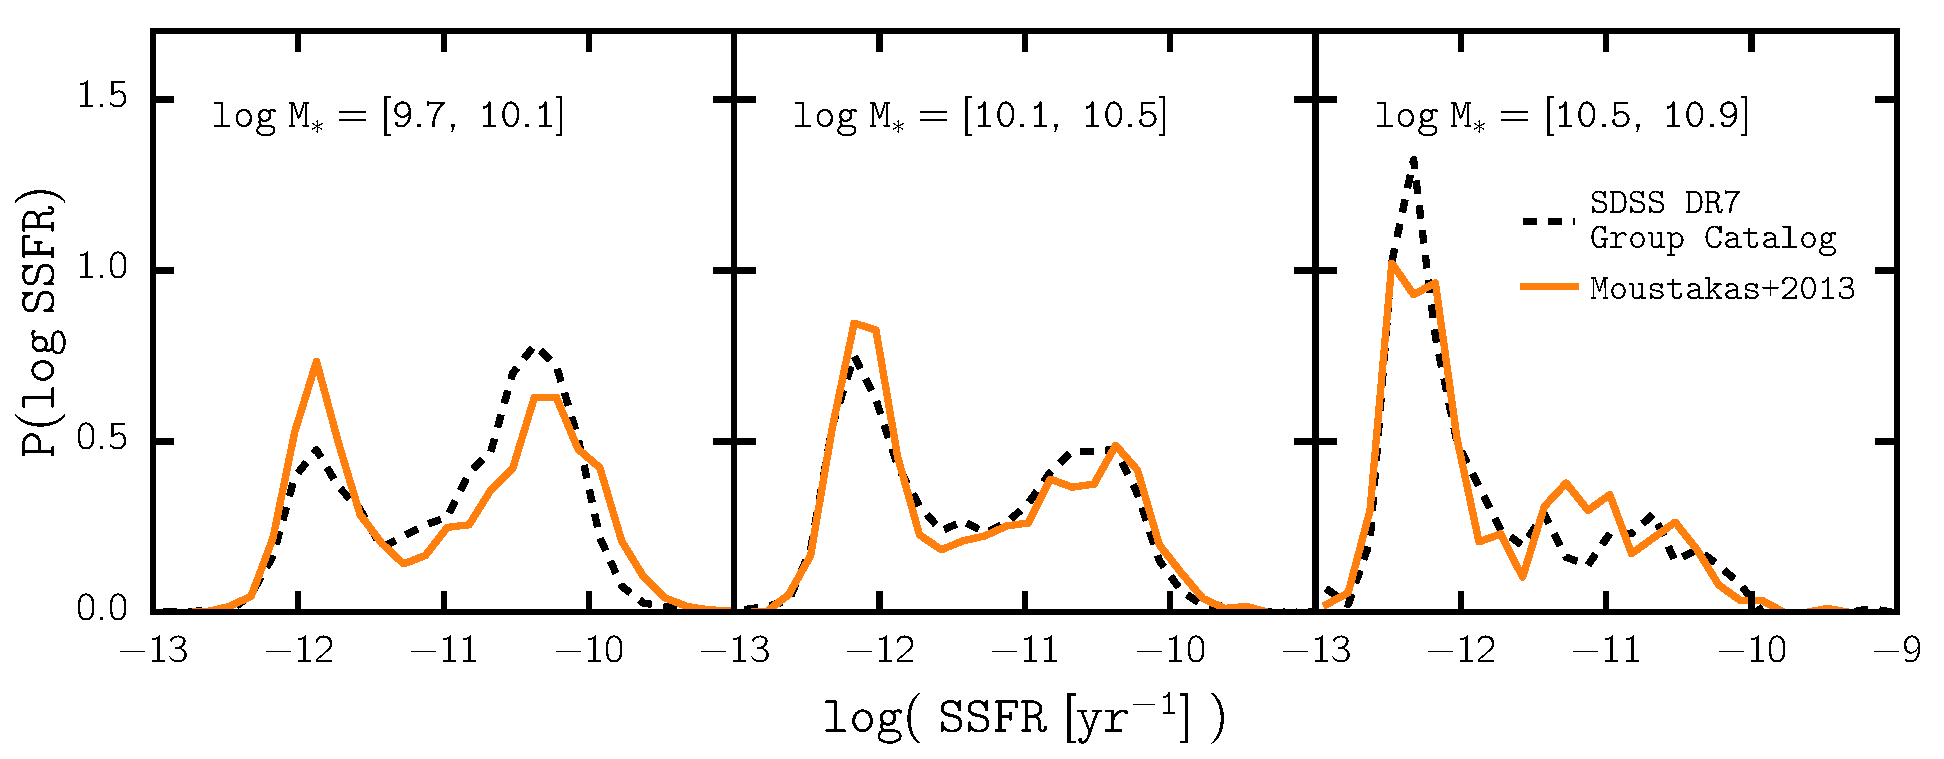
\includegraphics[width=\textwidth]{figs/cenq/Pssfr_comparison.pdf}
\caption{
Comparison of the SSFR distribution calculated using 
SSFRs from the SDSS DR7 group catalog (black dashed) versus
\cite{Moustakas:2013aa} (orange) for galaxies that are in 
both the SDSS DR7 group catalog and the \cite{Moustakas:2013aa} 
sample $z\sim0.1$ bin: $P(\mathrm{SSFR}^{\rm group})$ versus 
$P(\mathrm{SSFR}^{M2013})$. Galaxies are binned based on the
group catalog $\mathcal{M}_*$ for both distributions so that 
the same galaxies are examined in each bin. We impose SSFR 
bounds on $P(\mathrm{SSFR}^{M2013})$ for low SSFRs to reproduce 
the $P(\mathrm{SSFR}^{\rm group})$ quiescent peak (\S~\ref{sec:sdss}). 
We note that the M2013 sample does not contain a large number 
of galaxies within the group catalog's $z$ range at higher 
mass bins due its bright magnitude limit.
We find good overall agremeent between $P(\mathrm{SSFR}^{\rm group})$ 
and $P(\mathrm{SSFR}^{M2013})$. Furthermore, they have consistent 
green valley heights, which is the main feature of $P(SSFR)$ critical 
for constraining the central quenching timescale.
}
\label{fig:Pssfr_comp}
\end{center}
\end{figure*}

